\apendice{Plan de Proyecto Software}

\section{Introducción}
En este apartado se desarrollará la planificación temporal del proyecto, así como también un estudio de viabilidad.

\section{Planificación temporal}
Para la planificación temporal del proyecto, se sigue una metodología \english{Scrum}. Se realizarán diferentes \english{sprints}, en los que se marcaban objetivos. Idealmente, los \english{sprints} duran dos semanas. Debido a carga de trabajo externa a este proyecto, esta duración se ha visto afectada y se han realizado \english{sprints} de más y menos duración. . Durante cada uno de ellos, se irán creando y realizando las diferentes tareas correspondientes a los objetivos fijados en cada \english{sprints}. Al finalizar cada \english{sprint}, se realizan reuniones con los tutores para revisar los objetivos cumplidos y marcar unos nuevos. 

Se ha utilizado Github para el seguimiento de la aplicación, ayudados por el tablero Kanban de Zen-hub. Esta herramienta nos ha permitido llevar un seguimiento más detallado de la planificación en cada momento. El repositorio del proyecto, y las issues realizadas se encuentra en el \myurl{https://github.com/AdrianArnaiz/TFG-Neurodegenerative-Disease-Detection}{repositorio del proyecto}.

A su vez, cabe destacar que los primeros \english{sprints} no se muestran de manera correcta. Esto es debido al fallo de no cerrar los \english{sprints} en github, por lo que los gráficos \english{Burndown} están alterados.

\subsection{Sprint 1}
Idealmente, el comienzo de este sprint comenzaba el 15 de Diciembre. Debido a cargas de trabajo externas al proyecto, al final se comenzó el 14 de febrero. Duración del sprint: 14 de febrero 2019 al 28 de febrero 2019. Ver gráfico \english{Burndown} en la figura \ref{fig:sprint1}.
\imagen{sprint1}{Burndown chart del sprint 1}
Tareas realizadas:
\begin{itemize}
\item Instalación del cliente Github: GitTortoise.
\item Crear la estructura de directorios del repositorio.
\item Instalación de \LaTeX{} y todos sus componentes. 
\item Lectura en profundidad de dos artículos de Giovanni Dimauro: \cite{giovanni1} y \cite{giovanni2} . 
\end{itemize}
En este sprint se realizó la fase inicial del proyecto, que comprendía desde la instalación y creación de elementos principales, hasta la iniciación de la investigación.


\subsection{Sprint 2}
Duración del sprint: 28 de febrero de 2019 al 13 de marzo de 2019. Ver gráfico \english{Burndown} en la figura \ref{fig:sprint2}.
\imagen{sprint2}{Burndown chart del sprint 2}
Tareas realizadas:
\begin{itemize}
\item Realizar la taxonomía de las características extraídas de cada audio, qué características de cada tipo...
\item Identificar las herramientas de extracción de características de audio.
\item Realizar taxonomía de correspondencia entre las herramientas y las características concretas a extraer.
\item Realizar un arreglo en la preservación de privacidad de los audios del conjunto de datos.
\end{itemize}
En este sprint, seguimos explorando el estado del arte ahora de manera más precisa: empezar a ver en profundidad el proceso de extracción de características y medidas de los audios, explorando en diferentes artículos que características extraer y buscando las herramientas necesarias para su extracción.

\subsection{Sprint 3}
Duración del sprint: 13 de marzo 2019 al 29 de marzo 2019. Ver gráfico \english{Burndown} en la figura \ref{fig:sprint3}.
\imagen{sprint3}{Burndown chart del sprint 3}
Tareas realizadas:
\begin{itemize}
\item Búsqueda de audios, peticiones y realización de taxonomía de audios encontrados.
\item Lectura en profundidad de los artículos más importantes del estado del arte, i.e. \cite{Orz2016}.
\item Finalización de exploración del estado del arte: realizar taxonomía y resúmenes.
\end{itemize}
En este sprint se llevó a cabo la finalización de estado del arte y su resumen de aspectos y artículos más importantes. Un aspecto importante fue la búsqueda de audios, trabajo bastante arduo dentro del proyecto debido a que son muy difíciles de encontrar. Empezamos el proceso de extracción de características descrito en \cite{Orz2016}: instalación y familiarización de librerías, segmentación de audios, etc...

\subsection{Sprint 4}
Duración del sprint: 29 de marzo 2019 al 11 de abril 2019. Ver gráfico \english{Burndown} en la figura \ref{fig:sprint4}.
\imagen{sprint4}{Burndown chart del sprint 4}
Tareas realizadas:
\begin{itemize}
\item Instalar herramientas de manejo de audio como Disvoice.
\item Explorar el funcionamiento de estas herramientas.
\item Preprocesar los audios: eliminar silencios inicial y final.
\item Extracción de diferentes características de los audios con Disvoice.
	\begin{itemize}
    \item Extracción medidas prosódicas de audios completos.
	\item Extraer medidas de fonación de \english{voiced frames} de vocales y frase.
	\item Extraer medidas de articulación (cepstrales y de energía de transiciones).
	\end{itemize}
\end{itemize}
Se realizó el proceso de extracción de características. Se recorre toda la estructura de audios para crear las correspondientes matrices de características (en numpy) de cada tipo de audio y así dejar preparados los datos para entrenar modelos. Hay una matriz de características por cada tipo de audio y cada tipo de características. Para ello se realizó desde la instalación y comprensión del funcionamiento de las herramientas de manejo de audio, hasta extraer las medidas completas con la herramienta Disvoice.

\subsection{Sprint 5}
Duración del sprint: 15 de abril 2019 al 2 de mayo 2019. Ver gráfico \english{Burndown} en la figura \ref{fig:sprint5}.
\imagen{sprint5}{Burndown chart del sprint 5}
Tareas realizadas:
\begin{itemize}
\item Documentación de avances hasta el momento.
\item Realización de los \textbf{primeros experimentos} con clasificadores, incluyendo la limpieza de características necesaria para ello.
\item Realización proyección de características.
\item Investigación, documentación y aprendizaje sobre \english{Deep Learning}.
\end{itemize}
En este sprint, se documentó el trabajo realizado hasta el momento. También se realizó el estudio con clasificadores para los conjuntos de características extraídos con Disvoice. Probamos proyecciones de datos de estas características para graficarlos. En este sprint se comenzó la investigación y aprendizaje sobre Deep Learning, para su aplicación a posteriores sprints.


\subsection{Sprint 6}
Duración del sprint: 2 de mayo 2019 al 17 de mayo 2019. Ver gráfico \english{Burndown} en la figura \ref{fig:sprint6}.
\imagen{sprint6}{Burndown chart del sprint 6}
Tareas realizadas:
\begin{itemize}
\item Búsqueda de librerías de \english{Deep Learning} para audios.
\item Modificación de las características Disvoice.
\item División del conjunto de datos por sexo.
\item Realización de \textbf{segundos experimentos} con características Disvoice modificadas.
\end{itemize}
En este sprint realizamos la modificación de las características de Disvoice (adición de edad y sexo, división por sexos...) y realizamos los experimentos con estas nuevas características. También, siguiendo la línea del anterior sprint, profundizamos más en el \english{Deep Learning}, Buscando bibliotecas para la extracción de características de nuestros audios.

\subsection{Sprint 7}
Duración del sprint: 17 de mayo 2019 a 14 de junio 2019. Ver gráfico \english{Burndown} en la figura \ref{fig:sprint7}.
\imagen{sprint7}{Burndown chart del sprint 7}
Tareas realizadas:
\begin{itemize}
\item Arreglo de fallo encontrado.
\item Repetición de primeros y segundos experimentos: incluye repetición de análisis y resumen de resultados.
\item Instalación biblioteca VGGish (y VGGish2Keras).
\item Realizar extracción de características con VGGish (VGGish2Keras).
\item Realización \textbf{terceros experimentos} con características VGGish.
\item Análisis de viabilidad comercial: \english{lean canvas}.
\end{itemize}
En la reunión previa a este sprint, se revisó el código y encontramos un fallo de \concept{data snooping}. No hacíamos validación cruzada anidada (\english{nested CV}). Debido a esto, tuvimos que arreglar el error y repetir los experimentos realizados hasta el momento (primeros y segundos con características Disvoice). Tras finalizar, tuvimos que volver a analizar y resumir todos los resultados de los experimentos, aunque estos habían variado menos de lo esperado. También, siguiendo con la línea de anteriores sprints, realizamos la instalación de la biblioteca VGGish de \english{Deep Learning}, extrajimos las características de los audios con esta biblioteca y realizamos los experimentos con estas nuevas características. Para finalizar, y por pedido de la OTRI (Ofinia de transmisión de información de la Universidad de Burgos), se realizó un análisis de viabilidad comercial, concretamente un \english{lean canvas} de nuestro proyecto.

Cabe destacar que la duración de este sprint es bastante mayor de lo normal. Se debe a dos aspectos. El primero de ellos es que la carga de trabajo de este sprint era sustancialmente superior a los demás. Se debe a que en fallo encontrado requería de una repetición de gran parte del trabajo y además no podíamos frenarnos en los experimentos con \english{Deep Learning}. Por otra parte, coincidión con las dos últimas semanas del curso, las cuales estaban repletas de trabajos finales y exámenes de convocatoria, que hacían que el tiempo dedicado al proyecto tuviera que ser menor.

\subsection{Sprint 8}
Duración del sprint: 14 de junio 2019 a 24 de junio 2019. Ver gráfico \english{Burndown} en la figura \ref{fig:sprint8}.
\imagen{sprint8}{Burndown chart del sprint 8}
Tareas realizadas:
\begin{itemize}
\item Aprendizaje del patrón de diseño mediador-fachada.
\item Realización de la aplicación de escritorio.
\end{itemize}
En este sprint se realizó la aplicación demostrativa de escritorio. Para ello, se sugirió hacer mediante el patrón de diseño mediador-fachada. Por ello antes de realizar la aplicación se tuvo que comprender ese patrón. Una vez comprendido se realizó la aplicación. Como ya hemos comentado en la memoria principal, esta aplicación, aunque es la parte más vistosa, personalmente no la considero la parte más importante del proyecto. Únicamente es una aplicación que muestra una posible aplicación del resultado de este investigación, y que con las líneas de investigación futuras pudiera llegar a un producto funcional y estable.

\subsection{Sprint 9}
Duración del sprint: 24 de junio 2019 a 1 de junio 2019. Ver gráfico \english{Burndown} en la figura \ref{fig:sprint1}.
\imagen{sprint1}{Burndown chart del sprint 1}
Tareas realizadas:
\begin{itemize}
\item Revisión de la memoria hasta el momento.
\item Finalización de la memoria.
\item Búsqueda de documentación de pruebas unitarias en Minería de Datos.
\item Finalización de los anexos.
\end{itemize}
En este último sprint se hicieron las últimas tareas del proyecto. Se terminó toda la documentación, lo que comprendía desde revisar lo hecho anteriormente, realizar lo que faltaba por terminar y buscar información sobre pruebas unitarias en el campo de la minería de datos.


\section{Estudio de viabilidad}
En este apartado se abordará la viabilidad económica, comercial y legal de este proyecto.

\subsection{Viabilidad económica}
En este apartado, simularemos el coste del proyecto que tendría en una empresa, o en una venta al público.
\subsubsection{Coste personal}
Este proyecto cuenta con dos \textbf{profesores contratados} durante 6 meses para este proyecto. Por cada profesor se asignan 0,5 créditos, por lo que el coste\footnote{\url{http://www.ubu.es/sites/default/files/portal_page/files/pdi_laboral_2017_2.pdf}} por tutor consideramos que es el siguiente:
\begin{itemize}
\item Sueldo base mensual ayudante doctor: 1815,61 euros. 21787,32 euros anuales. En total imparte 24 créditos por lo que el coste anual por crédito es de 907,5 euros. El coste total es el siguiente:
\begin{equation}
907,5 \cdot 0,5 créditos = 453,75 euros
\end{equation}
\item Sueldo base mensual doctor permanente: 2325,24 euros. 27902,88 euros anuales. En total imparte 24 créditos por lo que el coste anual por crédito es de 1162.62 euros. El coste total es el siguiente:
\begin{equation}
1162.62 \cdot 0,5 créditos = 581,31 euros
\end{equation}
\end{itemize}

También cuanta con un desarrollador del proyecto. Supondremos un salario bruto de 2000 euros para el desarrollador. Habrá que tener en cuenta los \myurl{http://www.seg-social.es/wps/portal/wss/internet/Trabajadores/CotizacionRecaudacionTrabajadores/}{gastos de seguridad social}. 
\begin{itemize}
\item Cotización por parte de la empresa: 23.6\%
\item Cotización por parte del empleado: 4.7\%
\item \textbf{Total: 28.3\%}
\end{itemize}
Por lo tanto el coste del desarrollador se detalla en \ref{tabla:costespersonales}
\tablaSmallSinColores{Costes de personal}{p{6.4cm} p{2.15cm} p{8cm}}{costespersonales}{
  \multicolumn{1}{p{4.5cm}}{\textbf{Concepto}} & \textbf{Coste{}}\\
 }
 {
  Salario mensual neto  & \multicolumn{1}{r}{1217.25}\\
  Retención IRPF (15\%) & \multicolumn{1}{r}{216.75}\\
  Seguridad social  (28.3\%) & \multicolumn{1}{r}{566}\\
  Salario mensual bruto  & \multicolumn{1}{r}{2000}\\\hline
  \textbf{Coste total (6 meses)}  & \multicolumn{1}{r}{12000}\\\hline
  }


\subsubsection{Coste informático}

El coste informático es mínimo. Se ha utilizado un único portátil personal. Su coste fue de 800 euros y se supone una amortización de 5 años. Para ello se contabilizará únicamente el cose amortizado. 
\begin{equation}
(800 / (12 \cdot 5)) \cdot 6 = 80 euros
\end{equation}

\subsubsection{Ingresos}
Para este proyecto se ha contado con la concesión de la beca prototipos de la Oficina de Transmisión de Información de la Universidad de Burgos. La cuantía de la beca ha sido de 800 euros, por lo que estos serán los ingresos del proyecto.

\subsubsection{Coste Total}
El coste total se detalla en la tabla \ref{tabla:costetotal}

\tablaSmallSinColores{Coste Total}{p{6.4cm} p{2.15cm} p{8cm}}{costetotal}{
  \multicolumn{1}{p{4.5cm}}{\textbf{Concepto}} & \textbf{Coste{}}\\
 }
 {
  Coste desarrollador  & \multicolumn{1}{r}{12000}\\
  Costes Tutores(15\%) & \multicolumn{1}{r}{1035.06}\\
  Hardware & \multicolumn{1}{r}{80}\\\hline
  Beca prototipos  & \multicolumn{1}{r}{-800}\\\hline
  \textbf{Coste total (6 meses)}  & \multicolumn{1}{r}{12315.6}\\\hline
  }



\subsection{Viabilidad comercial}
Para analizar la viabilidad comercial, realizaremos un \english{lean canvas}, \ref{fig:LeanCanvas}, la cual es una herramienta de análisis de negocio desarrollada por Alex Osterwalder \cite{osterwalder2007business}.

\begin{figure}[!h]
		\centering
		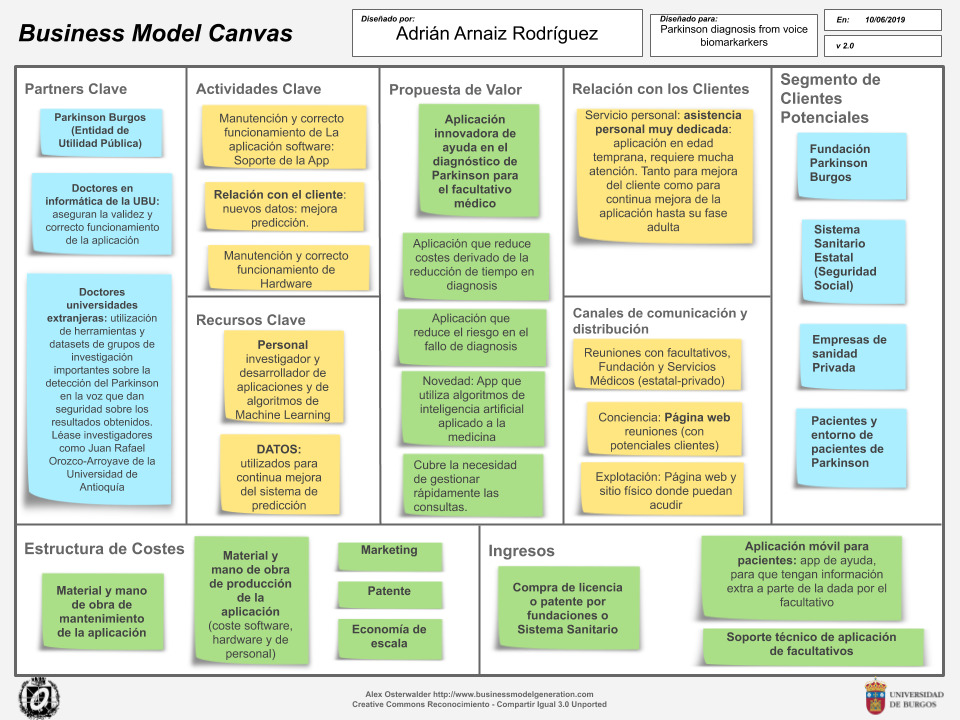
\includegraphics[width=1.1\textwidth]{LeanCanvas}
		\caption{Lean Canvas del proyecto}\label{fig:LeanCanvas}
\end{figure}


\subsection{Viabilidad legal}
Todo el código utilizado es de dominio público. Hemos utilizado multitud de librerías del lenguaje Python, las cuales son todas de dominio público. Las herramientas más concretas que hemos utilizado han sido las siguientes.
\begin{itemize}
\item \textbf{Disvoice}: alojado en \myurl{https://github.com/jcvasquezc/DisVoice}{repositorio público} de Github. \textbf{Tiene la licencia pública MIT}.
\item \textbf{VGGish}: alojado en \myurl{https://github.com/tensorflow/models/tree/master/research/audioset}{repositorio público de Github}.Pertenece al proyecto de Tensorflow. \textbf{Tiene la licencia pública Apache license 2.0}.
\end{itemize}
Todas las demás librerías utilizadas son propias de Python. También mencionar que no utilizamos el repositorio Disvoice original, sino que le hemos modificado para la ejecución en Windows. Esto ha sido posible ya que la licencia MIT permite tanto el uso comercial como la modificación el mismo.

